\documentclass[letterpaper,10pt,onecolumn,fleqn]{IEEEtran}
%draftclsnofoot

\usepackage{hyperref}
\usepackage{geometry}
\usepackage{tocloft}
\usepackage{color}
\usepackage{graphicx}
\usepackage{amsmath}

\geometry{margin=0.75 in}

\setlength{\parskip}{1em}
\setlength{\mathindent}{0pt}

%-------------------------- ASSIGNMENT 3: RELATIONAL ALGEBRA --------------------------%
\begin{document}

\noindent
Rhea Mae V. Edwards\\
CS 340, Fall 2017\\
Assignment 3

\section*{Relational Algebra}

\noindent
In this assignment you will be writing \underline{\textbf{\textit{relational algebra}}} (\underline{not SQL}) queries to select various sets of
data. Below is a schema of a auto dealership database.
\\ ~ \\ \noindent
Vehicle - The base class for types of vehicles to be sold.
\\ ~ \\ \noindent
Make - The brand of vehicle. (e.g. BMW, Ford etc)
\\ ~ \\ \noindent
Model - The specific model (2 Series, Focus etc). First production year is the first year that model was ever made.
\\ ~ \\ \noindent
Vehicle\_ Incentive - A relationship table between Vehicles and Incentives. Keeps track of when the incentive for that vehicle expires.
\\ ~ \\ \noindent
Incentive - Discounts and other deals. Type includes things like Factory or Dealer depending who is offering the incentive.
\\ ~ \\ \noindent
Inventory - The actual stock of vehicles in the lot. The price is the MSRP for that specific vehicle.
\\ ~ \\ \noindent
Color – The potential colors cars can come in. The name is the name given by the factory (Taffeta white).
The code is the hex representation of that color (e.g. \# FFFAFA)
\\ ~ \\

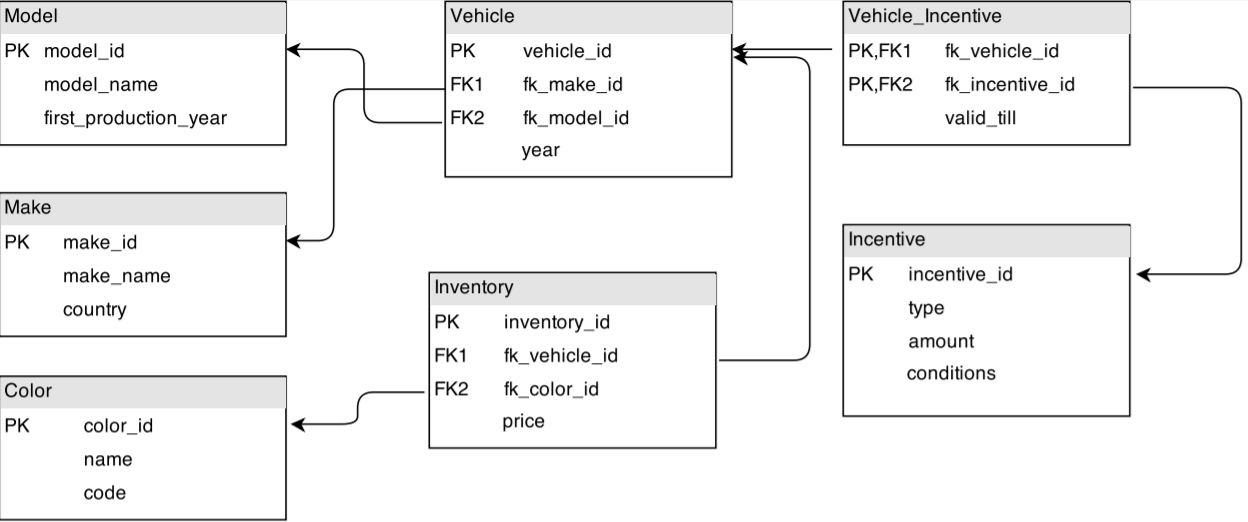
\includegraphics[width=\linewidth]{schema.png}

\newpage

\section*{Questions}

\begin{enumerate}

\item  
Select the make\_ name and model\_ name of all vehicles which have a first production year of 1976

\begin{flalign} 
\nonumber
\Pi_{Make.make\_ name, Model.model\_ name}  (\sigma_{Model.first\_ production\_ year = 1976} & 
\end{flalign}

\begin{flalign}
\nonumber
((Model \bowtie_{Model.model\_ id = Vehicle.fk\_ model\_ id} Vehicle)\bowtie_{Vehicle.fk\_ make\_ id = Make.make\_ id} Make))
& \\ \nonumber
\end{flalign} 

\item
Select the make\_ name and model\_ name of all vehicles with the color name Blue

\begin{flalign}
\nonumber
\Pi_{Make.make\_ name, Model.model\_ name} (\sigma_{Color.name = "Blue"} &
\end{flalign}

\begin{flalign}
\nonumber
((((Model \bowtie_{Model.model\_ id = Vehicle.fk\_ model\_ id} Vehicle) \bowtie_{Vehicle.fk\_ make\_ id = Make.make\_ id} Make) &
\end{flalign}

\begin{flalign}
\nonumber
\bowtie_{Vehicle.vehicle\_ id = Inventory.fk\_ vehicle\_ id} Inventory)  \bowtie_{Inventory.fk\_ color\_ id = Color.color\_ id} Color))
& \\ \nonumber
\end{flalign}

\item
Select the make\_ name, model\_ name and incentive amount for all vehicles with a dealer type incentive

\begin{flalign}
\nonumber
\Pi_{Make.make\_ name, Model.model\_ name, Incentive.amount} (\sigma_{Incentive.type = "dealer"} &
\end{flalign}

\begin{flalign}
\nonumber
((((Model \bowtie_{Model.model\_ id = Vehicle.fk\_ model\_ id} Vehicle) \bowtie_{Vehicle.fk\_ make\_ id = Make.make\_ id} Make) &
\end{flalign}

\begin{flalign}
\nonumber
\bowtie_{Vehicle.vehicle\_ id = Vehicle\_ Incentive.fk\_ vehicle\_ id} Vehicle\_ Incentive) &
\end{flalign}

\begin{flalign}
\nonumber
\bowtie_{Vehicle\_ Incentive.fk\_ incentive\_ id = Incentive.incentive\_ id} Incentive))
& \\ \nonumber
\end{flalign}

\item
Convert the following query to relational algebra\\

SELECT Player.id, Team.name, City.name FROM Player\\
INNER JOIN Team ON Player.team\_ id = Team.id\\
INNER JOIN City ON Team.city\_ id = City.id\\
WHERE Player.score = 100;

\begin{flalign}
\nonumber
\Pi_{Player.id, Team.name, City.name} (\sigma_{Player.score = 100} ((Player \bowtie_{Player.team\_ id = Team.id} Team) \bowtie_{Team.city\_ id = City.id} City))
& \\ \nonumber
\end{flalign}

\item
For problem 3 above, convert your relational algebra query into a SQL query.
\\ 

SELECT Make.make\_ name, Model.model\_ name, Incentive.amount FROM Incentive \\
INNER JOIN Vehicle ON Model.model\_ id = Vehicle.fk\_ model\_ id \\
INNER JOIN Make ON Vehicle.fk\_ make\_ id = Make.make\_ id \\
INNER JOIN Vehicle\_ Incentive ON Vehicle.vehicle\_ id = Vehicle\_ Incentive.fk\_ vehicle\_ id \\
INNER JOIN Incentive ON Vehicle\_ Incentive.fk\_ incentive\_ id = Incentive.incentive\_ id \\
WHERE Incentive.type = "dealer"

\end{enumerate}

\end{document}

